\chapter{PACORA Framework}

\begin{figure*}[p]
\center
\includegraphics*[width=1.2\columnwidth, angle=90]{Figures/pacora_framework_overview.pdf}
\caption{\label{pacora_arch_fig} Visual representation of \pacora's optimization formulation.  The runtime functions represented are the speech recognition, stencil kernel, and graph traversal applications from the evaluation Chapter~\ref{init_eval}.}
\end{figure*}

In this chapter, we describe the architecture of the PACORA framework.  We present the mathematical formulation and prove its convexity.  We also describe the two application specific-functions in detail and present experiments that helped guide the selection of the response-time function.


%present our initial evaluations of the potential of using \pacora for resource allocation in an operating system.

%------------------------------------------------------------------------------------------------------------------------------------------------------------------------
\section{\pacora Architecture}\label{sys_design}
%------------------------------------------------------------------------------------------------------------------------------------------------------------------------


\pacora is a framework designed to determine the proper amount of each
resource type to give each application. 

For our purposes an application is an entity to which the system
allocates resources: these can be a complete application (\emph{e.g.,}
a video player), a component of an application (\emph{e.g.,} a music
synthesizer), a background OS process (\emph{e.g.,} indexing), a job
in warehouse-scale computing, or a distributed application in a
distributed embedded system.

Resources are anything that the system can ``partition'' in hardware or software.  Resources can be thought of as typically as one of three types: compute, communication, and capacity\footnote{\pacora does not treat any resource types differently so classification is not strictly necessary. It is only described here to demonstrate the range of resources that could be controlled by \pacora.}.
In our operating system experiments, we use cores (compute), network bandwidth (communication), and cache ways and memory pages (capacity).
Other operating scenarios would have resources that perform similar functions at a different scale. For warehouse-scale computing, resources are more
likely to be different types of nodes, network bandwidth, and storage. For distributed embedded systems, resources would include compute devices, link bandwidths, and memories. 

\subsection{Resource Allocation as Optimization}

\pacora formulates resource allocation as an optimization problem
designed determine the ideal resource allocation across all active
application by trying to minimize the total penalty of the system. This approach is
analogous to minimizing dissatisfaction with the user experience
due to missed deadlines in a client system and minimizing the contract
penalties paid for violated SLAs in a cloud
system.   Figure~\ref{pacora_arch_fig} presents the formulation visually.

The optimization selects the allocations for all resources and
resource types at once.  This approach enables the system to make
tradeoffs between resource types.  For example, the system could
choose to allocate more memory bandwidth in lieu of on-chip cache, or
one large core instead of several small cores.  Given that all of the
resources allocated to an application contribute to the response time,
it would difficult to provide predictable response times for
applications without over-provisioning by independently allocating each resource type.

\pacora employs two types of application-specific functions in its optimization: a
response-time function (RTF) and a penalty function. The response-time
function represents the performance of the application with different
resources and is built with runtime measurements.  The penalty
function represents the user-level goals for the application
(\emph{i.e.,} the deadline and how important it is to meet) is set by the system, developer, or administrator.

A succinct mathematical characterization of this resource allocation scheme is the following:
\begin{eqnarray}
& \makebox[1in][r]{Minimize}   & \sum_{p\in P} {\pi_p(\tau_p(a_{p,1}\ldots a_{p,n}))} \label{op_eq1} \\
& \makebox[1in][r]{Subject to} & \sum_{p\in P} a_{p,r} \leq A_r, r = 1,\ldots n     \label{op_eq2}   \\
& \makebox[1in][r]{and}        & a_{p,r} \geq 0 \label{op_eq3}
\end{eqnarray}
Here $\pi_p$ is the penalty function for application $p$,
$\tau_p$ is its response time function,
$a_{p,r}$ is the allocation of resource $r$ to application $p$,
and $A_r$ is the total amount of resource $r$ available. 

\pacora is designed to be convex by construction to take advantage of efficient convex optimization methods for solving the optimization problem~\cite{BoVa}.



%------------------------------------------------------------------------------------------------------------------------------------------------------------------------
\subsection{Assumptions}
%------------------------------------------------------------------------------------------------------------------------------------------------------------------------
In Section~\ref{sys_design}, we have presented the mathematical framework behind \pacora.  However, in order to deploy \pacora in a real system, we also need to assume several things about the design of the system.  Here we describe these assumptions in detail.

\subsubsection{Hierarchical Scheduling}

\pacora is designed for systems where resource allocation is separated
from scheduling.  This split enables the use of application-specific
scheduling policies, which have the potential to be easier to design
and more efficient than general-purpose schedulers that have to work
for everything.  The resource allocation system is then able to focus on the
problem of \emph{how much} of each resource type to assign to each
application.  

In client machines, \pacora makes coarse-grain
resource-allocation decisions (\emph{e.g.,} cores and memory pages) at
the OS level, while the micro-management of these resources is left to user-level runtimes such as Intel
Threaded Building Blocks~\cite{CoMa08} or Lithe~\cite{lithe}, and to
user-level memory managers.  However, a user-level runtime is not strictly necessary: in Linux, for example, we have used \pacora to set thread affinity or size resource containers.

If the machine is operating in a cloud computing environment, \pacora could be used in a hypervisor to allocate
resources among guest OSes. For warehouse-scale computers, \pacora could be used to allocate
resources (\emph{e.g.,} nodes and storage) to jobs, while scheduling is
left to other entities such as the MapReduce framework\cite{mapreduce}
or the node OS.   

\pacora could be used in a system designed to consolidate realtime systems.  Resources can be allocated to various realtime user-level schedulers such as Earliest-Deadline-First or Rate-Monotonic schedulers, and \pacora will guarantee quality-of-service to the schedulers, eliminating the need in the case of many applications for a realtime OS designed around a single real-time scheduler.

\subsubsection{Allocation Enforcement}

\pacora relies on resource allocation mechanisms to assign resources and enforce allocations. For \pacora to be able to use a resource, the system must be able to allocate the resource (\emph{e.g.,} a core) or a fraction of it (\emph{e.g.,} a percentage of network bandwidth) to an application and enforce this allocation.  Enforcement can be in hardware or software.  For example, cache partitioning could be implemented in hardware easily by changing the replacement algorithm to limit what ways an application can write in to (as is done in our sandy bride prototype used in the experiments in Section~\ref{init_eval}) or the operating system could use page coloring emulate cache partitioning. 

We have found that these mechanisms are readily available in most systems for some resources (\emph{e.g.,} cores and memory pages) and can other can easily be managed in with software (\emph{e.g.,} network bandwidth).   During the course of this work we have also seen a QoS mechanisms being added to commercial systems (\emph{e.g.,} cache partitioning).
As more QoS mechanisms become available on future systems, other resources could be easily added to \pacora.

\subsubsection{Performance Isolation and Shared Resources}

\pacora assumes some amount of performance isolation between
applications.  In order for the RTFs to accurately reflect the
expected response times of the applications, it is important that the
response time does not change much as a function of the other
applications currently running on the machine.  However, the
performance isolation need not be completely perfect: all of our
evaluation was run on current x86 hardware with some shared resources,
and \pacora was still effective. Section~\ref{discuss} discusses
handling shared resources in more detail.


%------------------------------------------------------------------------------------------------------------------------------------------------------------------------
\section{Convex Optimization}\label{convex_sec}
%------------------------------------------------------------------------------------------------------------------------------------------------------------------------
If the penalty functions, response time functions, and resource
constraints were arbitrary, little could be done to optimize the total
penalty beyond searching at random for the best allocation.  However, we designed \pacora to be convex by construction, which enables us to use convex optimization~\cite{BoVa} methods to solve the optimization. 
By framing our resource allocation problem as a convex optimization problem, we get two significant benefits: for each problem an optimal
solution exists without multiple local extrema, and fast optimization methods with practical incremental solutions become feasible.  In this section, we prove the convexity of \pacora's optimization formulation.  The penalty and RTF function convexity are discussed in Sections \ref{PF_convexity} and \ref{RTF_convexity} respectively.  \pacora also formulates RTF \emph{creation} as a convex optimization
problem, as explained in Section~\ref{rtf_creation}.

\subsection{Resource Allocation Optimization Convexity}

A constrained optimization problem is \emph{convex} if both the objective function to be minimized
and the constraint functions that define its feasible solutions are convex functions.
A function $f$ is convex if its domain is a convex set and
$f(\theta x + (1-\theta)y) \leq \theta f(x) + (1-\theta)f(y)$
for all $\theta$ between 0 and 1.
A set is convex if for any two points $x$ and $y$ in the set, the point
$\theta x + (1-\theta)y$
is also in the set for all $\theta$ between 0 and 1.
If $f$ is differentiable, it is convex if its domain is an open convex set and
$f(y) \geq f(x) + \nabla f^T\cdot(y-x)$ where $\nabla f$ is the gradient of $f$.
Put another way, $f$ is convex if its first-order Taylor approximations
are always global underestimates of its true value.

A convex optimization problem is one that can be expressed in this form:
\begin{eqnarray*}
& \makebox[1in][r]{Minimize}   & f_0(x_1,\ldots x_m)                              \\
& \makebox[1in][r]{Subject to} & f_i(x_1,\ldots f_m) \leq 0, i = 1,\ldots k        \\
& \makebox[1in][r]{where}      & \forall i \quad f_i:\Re^m \rightarrow \Re \mbox{ is convex.}
\end{eqnarray*}


\pacora's resource allocation problem can be transformed into a convex
optimization problem in the $m = |P|\cdot n$ variables $a_{p,r}$ as
long as the penalty functions $\pi_p$ are convex non-decreasing and
the response-time functions $\tau_p$ are convex.  We designed our
functions to meet these constraints, and proofs of their convexity are shown below.
 
The resource constraints are affine and therefore convex; they can be rewritten as 
\begin{equation}
\sum_{p\in P} (a_{p,r} - A_r) \leq 0  -a_{p,r} \leq 0
\end{equation}
\begin{equation}
-a_{p,r} \leq 0
\end{equation}

The convex formulation makes the optimization scale linearly in the
number of resource types and the number of applications.  For client
operating systems with around 100 applications running and 10 resource
dimensions, the total number of variables in the optimization problem
is 1000---a very small problem which is solved in microseconds on
current systems.  Cloud systems could have many more than 100
applications running, but the problem size scales linearly and the
potential benefits of a good allocation should scale rapidly with the
size of the system.


%------------------------------------------------------------------------------------------------------------------------------------------------------------------------
\section{RTF Design}\label{RTFs}
%------------------------------------------------------------------------------------------------------------------------------------------------------------------------


In this section, we discuss the design considerations and requirements for \pacora's RTF, evaluate potential RTFs with different complexities, and describe the chosen design in more detail. Chapter~\ref{init_eval} evaluates the performance of the chosen RTF.  Chapter~\ref{discuss} discusses alternative and enhanced RTF models.

\subsection{Purpose}

In order for a resource allocation framework to make informed decisions about application performance, there must be a way for it to understand the performance impact of a resource allocation in the current system on the application's performance.  One can imagine several high-level approaches to accomplish this. One option would be for the the system to try a variety of allocations and select the best one.  However, there are a few disadvantages to this method: first, the system may need to try many points to find an efficient resource allocation for multidimensional allocation problems; second, the result for a single application may not compose well for multiple applications; and third, it doesn't give the system much understanding of the value of individual resources making resource tradeoffs difficult.  Another option would be something similar to hill climbing where the system incrementally adds or removes resources and measures the change in performance.  However, there are several challenges for an incremental approach as well.  Since the system relies on measuring the incremental gradients, it could get stuck in local minima or remain on a performance plateau for a particular resource without discovering the threshold that gives significant performance improvement (\emph{e.g.,} the point where the application fits in cache).  It could also be difficult to explore more than one resource dimension at a time. Additionally it could take quite a long time to reach an efficient resource allocation, particularly for a system with multiple applications running, and could violate the application's quality-of-service while exploring resource allocations.  While obviously these techniques can be improved upon, we felt the fundamental problems of composablity and potentially high overhead to find an efficient multidimensional allocation would be very difficult to overcome. 

For \pacora, we instead chose to take a modeling approach to represent an application's performance given its resource assignments.  We explicitly create RTFs from measured values that capture information about the performance impact of a particular resource to an application on the current hardware at a particular time. We chose to use models because they can be easily used in an optimization that considers multiple resources and applications at the same time. 

\subsection{Design Considerations}

When considering what was necessary for a performance model to be used in a real system we came up with the following requirements to guarantee that the model would be low cost to produce and use and work with real applications:
\begin{itemize}
\item Low cost to produce;
\item Low storage overhead;
\item Works with a variable number of resource dimensions;
\item Tolerant of noisy measurements;
\item Convex;
\item Easily computed gradients.
\end{itemize}

One approach to creating explicit resource-performance models would have been to model response times by recording past values and interpolating among them, however this idea has serious shortcomings for resource allocation problems:

\begin{itemize}
\item The multidimensional response time tables would be large and thus more expensive to measure and store;
\item Interpolation in many dimensions is computationally expensive thereby increasing the overhead of the resource allocation optimization;
\item The measurements will be noisy and require smoothing;
\item Convexity in the resources may be violated and as a result significantly increasing the cost of the resource allocation optimization by eliminating the opportunity to use efficient convex optimization techniques;
\item Gradient estimation will be slow and difficult.
\end{itemize}

Instead of interpolating, \pacora maintains a parameterized analytic response time model with the partial derivatives evaluated from the model \emph{a priori}. Application responsiveness is highly nonlinear for an increasing variety of applications like streaming media or gaming, thus requiring many data points to represent the response times without a model. Using models, each application can be described in a small number of parameters.  Models can be built from just a few data points and can naturally smooth out noisy data. Their gradients, needed by \pacora to solve the optimization problem efficiently, are easy to calculate. 

However, to realize the potential advantages of modeling we first needed to demonstrate that simple models could adequately represent the response time of an application for resource allocation purposes.  To determine if simple models would work and to select an appropriate model for \pacora's RTF functions, we used three steps.  First, we performed a simple study using microbenchmarks in a real system determine the complexity required for the model (presented in Section~\ref{init_model_eval}). Once we had determined the general form of the model from the experiments, we then designed a model that seemed logical using our domain knowledge of computer hardware, applications, and performance (explained in Section~\ref{final_rtf}).  Finally, we performed experiments using real benchmarks and kernels on a real system to validate that our model fit the measured values.  These final experiments and results are presented in Chapter~\ref{init_eval}.  

\subsection{Model Format Evaluation}\label{init_model_eval}

To test the potential of different model formats, we first performed a study comparing the accuracy of RTFs created from linear models, quadratic models, and genetically-programed response surfaces for 8 synthetic benchmarks and 5 phases of a real speech recognition kernel.   The RTFs studied use three resources dimensions: cores, off-chip memory bandwidth, and cache banks.  In this section, we describe these experiments and their results.

\subsubsection*{Applications}

\begin{table*}[t]
\centering
\scriptsize
\begin{tabular}{|l|c|c|c|l|}
\hline
 Name  & Processor  &  Cache &  Offchip BW & Description \\ \hline
 p+c+b+ & benefits & benefits & benefits &  Copies data from large blocks, with reuse (multithreaded)\\ \hline
p--c+b+ & oblivious & benefits & benefits &  Copies data from large blocks, with reuse (single threaded)\\ \hline
p+c--b+ & benefits & oblivious & benefits &  Streaming copies with no reuse (multithreaded)\\ \hline
p--c--b+ & oblivious & oblivious & benefits &  Streaming copy with no reuse (single threaded)\\ \hline
p+c+b-- & benefits & benefits & oblivious &  Copies data repeatedly from large blocks (multithreaded)\\ \hline
p--c+b-- & oblivious & benefits & oblivious &  Copies data repeatedly from a large block (single threaded)\\ \hline
p+c--b-- & benefits & oblivious & oblivious &  Pointer chases through long lists (multithreaded)\\ \hline
p--c--b-- & oblivious & oblivious & oblivious &  Pointer chases through a long list (single threaded)\\ \hline
\end{tabular}
\caption{Synthetic microbenchmark descriptions. Each benchmark captures a different combination of responses to resource allocations.  ``Benefits'' means that application performance improves as more of that resource is allocated to it (though sometimes only up to a point).  ``Oblivious'' means that the application performance barely improves or does not improve at all as more of that resource is allocated to it.}
\label{table:benchmarks1}
\end{table*}

\begin{table*}[t]
\centering
\scriptsize
\begin{tabular}{|c|c|l|l|}
\hline
 Phase  & Name & Description & Behavior \\ \hline
 1 & Cluster  & Compute probability, step 1 &  Accumulate, up to 6 MB data read, 800KB written\\ \hline
 2 & Gaussian  & Compute probability, step 2 &  Calculate, up to 800KB read, 40KB written\\ \hline
 3 & Update & Non-epsilon arc transitions &40KB read, small blocks, dependent on graph connectivity\\ \hline
 4 & Pruning & Pruning states & Small blocks, dependent on graph connectivity\\ \hline
 5 & Epsilon & Epsilon arc transitions & Small blocks, dependent on graph connectivity\\ \hline
\end{tabular}
\caption{Description of phase behavior in LVSCR application.}
\label{table:app}
\end{table*}

We created a set of synthetic microbenchmarks specifically designed to evaluate our modeling techniques by representing the space of possible resource behaviors in 3 dimensions.  Table \ref{table:benchmarks1} describes these benchmarks.  In general, each benchmark represents a generic category of behavior that we might expect to see in phases of real applications.  We classified the benchmarks based on whether they benefit from additional processor, cache or bandwidth resources, or whether they derive no benefit from running on a large allocation of a given resource.  We also limited the size of the benchmarks along these resource dimensions so that they encounter performance cliffs on our simulated machine.  For example, a benchmark's performance might benefit from additional cores up to 4 cores but not from more than 4 cores.   Parallel benchmarks were parallelized with \texttt{pthreads}~\cite{pthreads}.  The benchmarks each run an average of 1.9 billion cycles per execution.

We also evaluated a real multithreaded application with multiple phases of behavior, specifically
a Hidden-Markov-Model (HMM) based inference algorithm that is part of a large-vocabulary continuous-speech-recognition (LVCSR) application \cite{chong-eama08, huang-speech}. This application case study demonstrates the varying ability of our models to capture real application behavior.

LVCSR applications analyze a set of audio waveforms and attempt to distinguish and interpret the human utterances contained within them. The recognition network we used here models a vocabulary of over 60,000 words and consists of millions of states and arcs. The inference process is divided into a series of five phases, and the algorithm iterates through the sequence of phases repeatedly with one iteration for each input frame. Table~\ref{table:app} lists the characteristics of each phase of the application.  Each phase runs for an average of 24 billion cycles per execution.

\subsubsection{Resources}
To properly test the potential RTF functions, we implement hardware partitioning mechanisms for three of most important shared on--chip resources.  We specifically chose one of each of the resource types described in Section~\ref{sys_design}; we provide partitioning mechanisms for cores (compute), interconnect bandwidth to DRAM (communication), and L2 cache capacity (capacity).

\paragraph{Core Pinning}
To partition cores, our implementation uses the thread affinity feature built into the Linux 2.6 kernel. We restrict the threads belonging to an application to run on the cores assigned to that application.  We assume a homogeneous collection of cores, and that only last level caches are shared among applications, which means that there is nothing to differentiate a core from any other when they are being allocated.

\paragraph{Globally Synchronized Frames}
To partition off-chip bandwidth, we use the Globally Synchronized Frames (GSF) approach presented in Lee et al. \cite{gsf}.  We chose this approach because it does not require complex hardware modifications, provides strict QoS guarantees for minimum bandwidth and the maximum delay of the network, and provides proportional sharing of excess bandwidth.  GSF controls the number of packets that a core can inject into the network per frame, and each core is guaranteed to get the number of packets allocated to it each frame.  GSF enables cores to inject packets into future frames if their current allocation is already exceeded. This allows excess bandwidth to be shared among cores proportional to their packet allocation.  To simplify prediction by making performance more deterministic, our current implementation does not make any future frames available during training, meaning that applications get exactly their allocation each frame.

\paragraph{Cache Partitioning}
 We implemented bank-based cache capacity as opposed to way-based partitioning to preserve cache associativity in our machine.  We assumed banks are sized at 1 MB, and we assume no additional overhead to lookup the correct bank.  Our experiments do not reallocate banks during execution, so we did not add a reallocation overhead either.

\subsubsection*{Modeling Techniques}
We use multivariate regression techniques to create explicit statistical models for predicting the performance of an application given a resource allocation of a particular size.  We create one regression model per performance metric per application phase.

Linear least-squares regression techniques produce simple models that can be expressed concisely and are therefore more portable. Linear regression techniques can outperform nonlinear ones when training sets are small, the data has a low signal to noise ratio, or sparse sampling is used\cite{hastie}. These criteria apply in our case. These models are attractive due to their simplicity, but their restricted expressiveness may reduce their accuracy of the underlying system.

Linear models may be realized in varying forms (i.e. it is the combination of terms that is linear, rather than the degree of each term).  The simplest models are linear additive models, which take the form:

\begin {equation}
y(x) = a_0 + \sum_{i=1}^{N}{a_ix_i}
\end {equation}

Multivariate linear additive models contain one term for each variable (i.e. an allocation, $x_i$) and an intercept term ($a_0$).  The regression tunes the coefficient associated with each term ($a_i$) to fit the sample data as accurately as possible.  Note that the linear additive model has no way to represent any possible interaction between the variables, implying that all variables are independent---which is expressly not true in our scheduling scenario.  For example, a smaller cache size will result in increased cache misses and an increased demand for memory bandwidth, meaning that the effect of a change in bandwidth allocation is not independent from a change in cache size in terms of its effect on performance.  However, there interactions may be small enough in practice to ignore in the model.

More complex multivariate linear regression models often include terms for variable interaction and polynomial terms of degree 2 or more.  Such models are commonly termed {\em response surface models} and have the general form:

\begin {equation}
y(x) = a_0 + \sum_{i=1}^{N}{a_ix_i} + \sum_{i = 1}^{N}\sum_{j=i}^{N}{a_{ij}x_ix_j} + ...
% \sum_{i=0}^{N}{a_{ii}x_i^2}
\end {equation}

These polynomial models capture more complex dependencies between the input variables.  However, we as modelers must still explicitly express the nature of the relationship between input and output in the form we give the polynomial equation.

Selecting the best possible equation form for the data automatically requires the use of nonlinear regression techniques such as local regression, cubic splines, neural networks, or genetic programming \cite{alvarez-thesis, bodik-acdc09, wasserman-book}.  The disadvantage of these techniques is that the models may create difficulties for analytic maximization algorithms.
%LOESS models have been used in the past in situations where the models must be retrained online as more data points are collected from the running system \cite{bodik-acdc09}.

Genetic programming is a technique, based on evolutionary biology, used to optimize a population of computer programs according to their ability to perform a computational task. In our case, the `program' is an analytic equation whose evaluation embodies a response surface model, and the `task' is to match sample data points obtained from full--scale simulations \cite{alvarez-thesis}. The output, termed a
{\em genetically-programmed response surface} (GPRS), are nonlinear models that create explicit equations describing the relationship between design variables and performance, and we incorporate them into our framework as an example of a nonlinear modeling alternative.
A GPRS is generated automatically, meaning that the modeler does not have to specify the form of the response surface equation in advance. Instead, genetic programming \cite{koza} is used to create an equation and tune the coefficients.  For more information on GPRS creation, see \cite{alvarez-thesis} or \cite{cook-dac08}.

We also explored a statistical machine learning technique, Kernel Canonical Correlation Analysis (KCCA) \cite{kcca}, to predict the response time in the style of \cite{Archana}. However, the results are not presented here as we found that we generally had too few sample points for the models to function.

\subsubsection*{Experimental Testbed}
We use Virtutech Simics \cite{simics} to simulate a CMP system with a two level on-chip memory hierarchy to collect the data used create our performance models and to test the effectiveness of our resource scheduling framework.  Simics is a full system simulator capable of running a commodity OS and completing simulations consisting of billions of cycles. We modify the Simics cache and memory timing modules to reflect the capabilities of our hardware partitioning mechanisms.  Our target machine has 10 cores, private 64KB L1D and 32KB L1I caches for each core and a shared L2 (16 MB, 16-way set associative).  All caches have 128 B lines.   All banks in the L2 cache have uniform access time of 7 cycles.  Our target machine runs Fedora Core 5 Linux (kernel 2.6.15). We constrain the simulated system to a maximum allocation of 10 cores, 16 MB of L2 cache, and 4 cache lines/cycle of off-chip bandwidth, and a minimum allocation of 1 core, 16 KB of L2 cache, and 5 cache lines/thousand cycles of off-chip bandwidth.


\subsubsection*{Evaluation of Model Accuracy}

To test the accuracy of the different model types, we chose a sample of 55 points from the space of 19200 possible allocations (or 0.3\%) using an Audze-Eglais Uniform Latin Hypercube design of experiments~\cite{bates-aes03}, and trained the models using this sample set. Audze-Eglais selects sample points which are as evenly distributed as possible through the space of possible allocations  We then evaluated the accuracy of the model relative to measured performance on a training set which contains all points disjoint from the sample set.  %Due to the length of our simulations, we could not exhaustively compare to all possible allocations and so limited our model error analysis to a testing set of 10 randomly selected points.  

\begin{table}\centering
\small
\begin{tabular}{|l|c|c|c|}
\hline
Name & Linear & Quadratic & GPRS \\ \hline
 p--c--b-- & 0.06\% (0.04) & 0.04\% (0.04) &0.02\% (0.02) \\ \hline
 p--c--b+ &   234.07\% (287.44) & 139.21\% (167.10) &  0.23\% (0.40)   \\ \hline
 p--c+b-- &  12.67\% (5.30) &  8.26\% (5.30) &  0.02\% (0.02) \\ \hline
 p--c+b+ &  12.04\% (5.09) &  7.83\% (4.69) & 0.06\% (0.06)  \\ \hline
 p+c--b-- &  0.07\% (0.05) &  0.05\% (0.06)  &  0.05\% (0.03)  \\ \hline
 p+c--b+ &  271.05\% (377.53) & 164.23\% (226.23) & 0.51\% (1.08) \\ \hline
 p+c+b--&  13.08\% (6.91) & 8.79\% (7.32) & 0.06\% (0.07) \\ \hline
 p+c+b+&  12.07\% (4.86) &  8.05\% (5.49) & 0.08\% (0.06)  \\ \hline
   \end{tabular}
 \caption{Means (standard deviations) of percentage error in runtime cycles for each of the predictive models for each of the synthetic microbenchmarks.}
\label{table:acc-cycles}
\end{table}


Table~\ref{table:acc-cycles} reports the mean and standard deviation of percentage error for the synthetic benchmarks of each of the models in predicting runtime cycles of each allocation versus the actual measured performance of that allocation.  We can see that two of the benchmarks, p+c--b-- and p--c--b--, seem to be very easy to predict and all three model types have less than 0.1\% mean error.  Four of the remaining benchmarks, p--c+b--, p--c+b+, p+c+b--, and p+c+b+, are more difficult to predict for the linear and the quadratic model. The linear model has an error around 12\% with a significant standard deviation, 5\%, for each benchmark.  The quadratic model performs a bit better and has an average error around 8\% for each of these benchmarks but still has a very large standard deviation.   The GPRS model, however, performs extremely well on these benchmarks and again has an average error of less than 0.1\%.  The final two benchmarks, p--c--b+ and p+c--b+, prove quite challenging for the linear and quadratic model resulting in an average error of 250\% and 150\% respectively.  The GPRS model, however, has very little trouble with these benchmarks and produces an error around 0.5\%.

Figure~\ref{fig:acc} visually represents what is happening in each of the these cases.  The figure plots the predictions from each model versus measured data for all the benchmarks.  The x axis is resource configurations ordered by runtime and the y axis is the runtime.   Looking at the plots we can see that the benchmarks that all models perform well on have a very predictable structure and no performance cliffs.  In particular benchmarks which encounter a cliff and then saturate (such as the working set fitting in cache) prove difficult for the linear and quadratic models.
 
 %It is also worth noting that the amount of error introduced in the linear additive and quadratic model causes them to predict negative values for some benchmarks.

\begin{figure*}
	\centering
	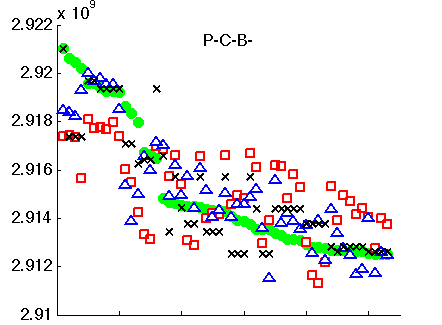
\includegraphics[scale = 0.34] {Figures/ooo_trainpredplot.png}
	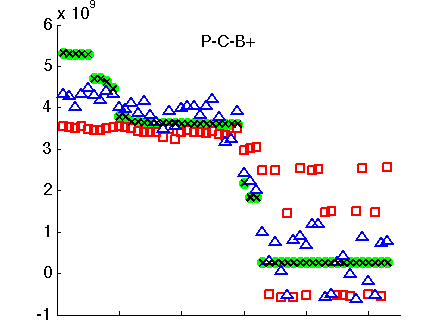
\includegraphics[scale = 0.34] {Figures/oop_trainpredplot.png}
	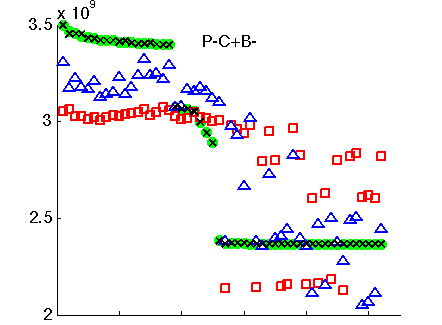
\includegraphics[scale = 0.34] {Figures/opo_trainpredplot.png}
	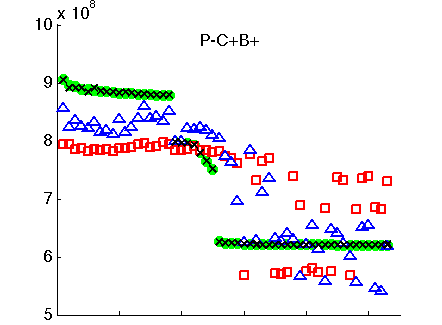
\includegraphics[scale = 0.34] {Figures/opp_trainpredplot.png}
	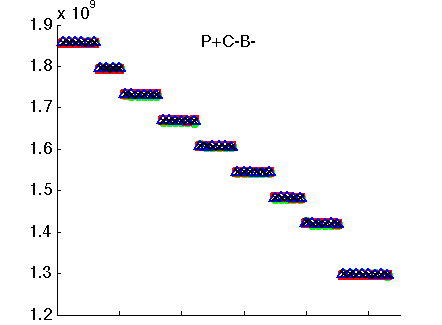
\includegraphics[scale = 0.34] {Figures/poo_trainpredplot.png}
	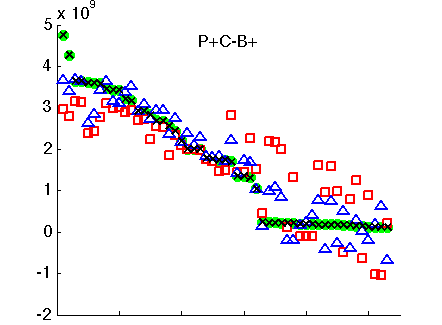
\includegraphics[scale = 0.34] {Figures/pop_trainpredplot.png}
	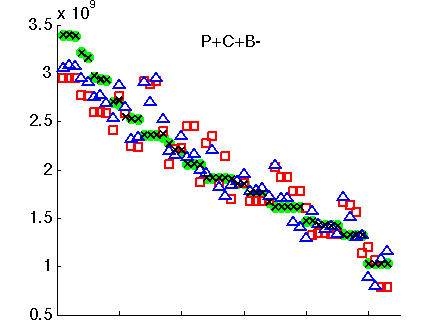
\includegraphics[scale = 0.34] {Figures/ppo_trainpredplot.png}
	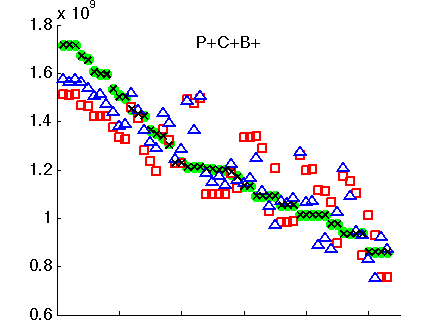
\includegraphics[scale = 0.34] {Figures/ppp_trainpredplot.png} \\
	
\includegraphics[scale = 0.5] {Figures/acc_comp_legend_horz.png}
	\caption{ \small Comparison of model accuracy for the eight microbenchmarks when predicting runtime in cycles. Each point represents a prediction for a machine configuration, and points are ordered along the x-axis based on decreasing measured run time. Y-axis plots predicted or measured runtime in cycles; note the differing ranges. In most cases, the nonlinear GPRS--based model is so accurate that it precisely captures all sample points.}
	\label{fig:acc}
\end{figure*}



\begin{table}\centering
\small
\begin{tabular}{|l|c|c|c|}
\hline
Name & Linear & Quadratic & GPRS \\ \hline
 cluster &  4.27\% (3.66) & 6.90\% (5.67)  & 15.52\% (10.36)  \\ \hline
 gaussian&  1.83\% (0.72) & 4.16\% (2.49) & 2.33\% (3.19)  \\ \hline
 update&  4.98\% (3.04) & 7.94\% (7.12)  & 5.89\% (5.09)  \\ \hline
 pruning&  2.27\% (1.08) & 10.70\% (10.29)  & 3.07\% (2.91)  \\ \hline
 epsilon &  3.88\% (4.01) & 4.66\% (4.27)  & 2.69\% (1.09)  \\ \hline
   \end{tabular}
 \caption{Means (standard deviations) of percentage error in runtime cycles for each of the predictive models for each of the phases of the LVSRC application.}
\label{table:acc-cycles-lvsrc}
\end{table}


While certain benchmarks are more challenging than others, there is no substantial difference in prediction accuracy between the synthetic benchmarks and real application. Table~\ref{table:acc-cycles-lvsrc} shows the accuracy of predictions of runtime (in cycles) per phase in terms of percentage error when measured against a test set.  The phases of the LVSRC application were actually more easily predicted than some of the microbenchmarks.  Due to the extreme length of the application (which was run to completion), the space of allocations we considered was limited to a maximum of two cores.  We reduced the size of the sample set correspondingly.  As a result, Table~\ref{table:acc-cycles-lvsrc} reflects models tuned on very small samples; with some adjustment of the genetic search parameters to prevent overfitting, all of the GPRS--based model percentage errors were reduced below 2\%.

%%For all of the applications, we can see that the models captured the performance of 90\% of the test points with less than []\% error.  This result leads us to believe that the model is an adequate enough representation of application performance to be useful in predicting performance for the remainder of the allocation options.

Clearly, the nonlinear models are extremely accurate and would make excellent input to our spatial resource allocation algorithm.  However, the GPRS--based models used here took between 0.5 and 6 hours each to build, so clearly they would have to be created offline and stored for use at runtime.  The linear models can be trained extremely rapidly, but are less accurate.  The true metric of whether or not a model is accurate ``enough'' depends on the quality of the decisions made based on it.


\subsubsection*{Effect of Sample Size on Model Accuracy}
\label{sec:eval:acc-sample}

Figure ~\ref{fig:acc-sample} shows the impact that changing the sample set size has on model accuracy, using the example of execution time predictions for the microbenchmarks.  It is worth noting that while the accuracy of the quadratic and  nonlinear models improve rapidly with increasing sample size, the linear additive model sees no improvement on average.  This failure to improve when exposed to additional data indicates that it is the {\em form} of the model itself which is flawed (i.e. too simplistic).  Another important feature is that as sample size increases, the improvement seen by the other models slows, indicating a point of diminishing returns for increasing sample size.

This sample size analysis informs our decision about whether we can afford to use online or offline, linear or nonlinear models.  On the one hand, GPRS--based nonlinear models are much more accurate even when given smaller sample sizes.  However, they take a long time to train, and cannot be rapidly adapted to account for new data points.  On the other hand, linear models of sufficient complexity require more points to succeed, but can be rapidly trained and retrained.  A hybrid approach, in which genetic programming is used to construct the form of the response surface model offline, and then the model's coefficients are retuned based on performance data collected online, may a viable way to get the best of both worlds.

\begin{figure}
	\centering
	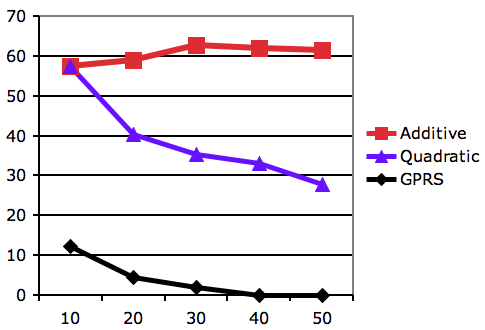
\includegraphics[scale = 0.5] {Figures/acc_sample.png}
	\caption{ \small Comparison of model accuracy for different models as training sample size is increased.  Y-axis is average percentage error in predictions of runtime averaged across all benchmarks. X-axis is increasing sample size.  Some models are more robust to reduced sample size than others.}
	\label{fig:acc-sample}
\end{figure}


\subsection{Response-Time Functions}\label{final_rtf}

Response-time functions (RTF) represent the expected \emph{response
  time} of an application as a function of the resources allocated to
the application. The response time is an application-specific measure
of the performance of the application.  For example, the response time
of an application might be:
    \begin{itemize}\itemsep0pt \parskip0pt \parsep5pt
    \item The time from a mouse click to its result;
    \item The time to produce a frame;
    \item The time from a service request to its response;
    \item The time from job launch to job completion;
    \item The time to execute a specified amount of work.
    \end{itemize}

The RTFs are built to be convex functions.  All applications have a
function of the same form, but the application-specific weights are set
using the performance history of the application.  RTFs are designed
to capture information such as how well an application scales with a
particular resource. As a result, RTFs naturally support
heterogeneity.  Each CPU or GPU type is simply viewed as a different
resource type by the system, and thus the RTFs will represent how
effectively an application uses a particular type of
core. Figure~\ref{sample_rtf} shows two example RTFs we have created
from applications we studied.

\begin{figure*}[hb]
\subfloat{
\includegraphics*[bb=0 0 360 360,width=.48\columnwidth]{Figures/bfs-fig.pdf}
\label{bfs-fig}
}
\subfloat{
\includegraphics*[bb=0 0 360
  360,width=.48\columnwidth]{Figures/streamcluster-fig.pdf}
\label{streamcluster-fig}
}  
\caption{\label{sample_rtf} Response-Time Functions for a
  breadth-first search algorithm and \texttt{streamcluster} from the PARSEC benchmark suite~\cite{parsec}. We show two resource dimensions: cores and cache ways.}
\end{figure*}

Equation~\ref{rtf_eq} below shows the RTF we selected for \pacora.  

\begin{equation}\label{rtf_eq}
\tau(w,a) = \tau_0 + \sum_{i\in n,j\in n}{\frac{w_{i,j}}{\sqrt{a_i * a_j}}}
\end{equation}

Here $\tau$ is the response time, $i$ and $j$ are
resource types, $n$ is the total number of resource types,
$a_{i}$ and $a_{j}$ are the allocations of resource types $i$
and $j$, and $w_{i,j}$ is the application-specific weight for
the term representing resources $i$ and $j$.

In our experience the cross term weights (those with $i\neq j$) are almost always negligible and can be omitted if desired.
This omission allows the dimensionality of the function, and thus the storage space required, to increase roughly linearly with the number of resource types.  The value of the cross terms is discussed further in Chapter~\ref{init_eval}.

We chose this specific function because it is convex in the resources, and in initial application studies,
we found it models response time behavior accurately enough to allow the optimization to make good decisions. Section~\ref{RTFs} describes the design considerations for the RTFs in more detail. Chapter~\ref{init_eval} shows these evaluation results and discusses alternative models that were considered and evaluated during the design process.

As explained in Section~\ref{convex_sec}, \pacora models response times with functions that are convex by construction in order to take advantage of the efficient solution methods available in convex optimization.
The specific function chosen for \pacora is shown in Equation~\ref{rtf_eq} above.
In this equation, the response time is modeled as a weighted sum of component terms,
roughly one per resource, where a term $w_i/a_i$ is the amount of work $w_i \geq 0$ divided by $a_i$, the allocation of the $i$th resource~\cite{Snav}.  We felt that this naturally represented approximately how resources behave. For example, one term might model instructions executed divided by total processor MIPS, so the application-specific $w$ \pacora is learning is the number of instructions.  As we increase the allocation of MIPS, then we'll see the contribution to total runtime from this term decrease since the additional processing power reduces the time to execute the instructions.  Other terms follow the same pattern but for different resources such as model network accesses divided by bandwidth, and so forth.

The examples described above all contain only a single resource type.  However, our intuition was that there may be relationships between resource types and asynchrony and latency tolerance may make response time components overlap partly or fully. For example, one can easily imagine that the amount of cache an application has affects its required memory bandwidth.  Thus we added additional terms to represent the interactions between resources.  To our surprise, in most of our experiments, we have found that the interaction terms are nearly always negligible and thus can be eliminated to save space and computation.  However, it is possible that some systems would still require them.  Interaction term results are shown in Chapter~\ref{init_eval}.   

It is obviously important to guarantee the positivity of the resource allocations. This guarantee can be enforced as the allocations are selected during penalty optimization, or the response time model can be made to return $\infty$ if any allocation is less than or equal to zero. This latter idea preserves the convexity of the model and extends its domain to all of $\Re^n$ and consequently we used this approach in our implementation.

Our chosen model design satisfies the design requirements listed above.  The model is low cost to produce: we can use convex optimization to produce it, which is described in Chapter~\ref{tess_design_ch}. The models (without the interaction terms) scale linearly with the number of resource dimensions and only require a small number of history values to produce a good model so they are lightweight to store.  They can capture information about all of the resource types and are tolerant of noise (See Chapters~\ref{init_eval} and \ref{discuss} for variability results and discussion) . Such models are automatically convex in the allocations because $1/a$ is convex for positive $a$ and because a positively-weighted sum of convex functions is convex.  Lastly,
the gradient $\nabla\tau$, which is needed by the penalty optimization algorithm, is simple to compute since $\tau$ is analytic, generic, and symbolically differentiable.


\subsection{Response Time Convexity}\label{RTF_convexity}

\begin{figure*}[h]
\center
\includegraphics*[width=.80\columnwidth]{Figures/dedup_5hp.png}
\caption{\label{dedup_outlier_fig} Measured runtimes for the dedup benchmark in PARSEC varying cores from 1-8 and giving 1, 2, and 12 cache ways. Ways 3-11 are not shown, but look nearly identical to 2 and 12.}
\end{figure*}

\begin{figure*}[h]
\center
\includegraphics*[width=.80\columnwidth]{Figures/mem_page_data.png}
\caption{\label{mem_page_fig} Average frame time for an n-bodies application running on Windows 7 while varying the memory pages and cores.}
\end{figure*}


We now show that response time functions $\tau$ are convex
in the resources $a_i$ given any of the possibilities we have considered.
%Since norms preserve convexity, this reduces the question to proving each term in the norm is convex.
%Since all quantities are positive and both maximum and scaling by a positive constant preserve convexity,
%\begin{eqnarray*}
%\lefteqn{w/(b\cdot\min(c_1\alpha_1(m),c_2\alpha_2(m)))}   \\
%&=& \max(w/(b\cdot c_1\alpha_1(m)),w/(b\cdot c_2\alpha_2(m))).
%\end{eqnarray*}
%It therefore only remains to show that both $1/\sqrt{b\cdot m}$ and $1/(b\cdot\alpha(m))$ are convex in $b$ and $m$.

A function is defined to be \emph{log-convex} if its logarithm is convex.
A log-convex function is itself convex because exponentiation preserves convexity,
and the product of log-convex functions is convex because the log of the product is the sum of the logs,
each of which is convex by hypothesis.
Now $1/a$ is log-convex for $a > 0$ because $-\log a$ is convex on that domain.
In a similar way, $\log(1/\sqrt{a_i\cdot a_j}) = -(\log a_i + \log a_j)/2$
and $\log a^{-1/d} = -(\log a)/d$ are convex, implying $\log(1/\sqrt{a_i\cdot a_j})$ and $\log a^{-1/d}$ are also.
Finally, $\log (1/\log a)$ is convex because its second derivative is positive for $a > 1$:
\begin{eqnarray*}
\frac{d^2}{da^2}\log (1/\log a) &=& \frac{d^2}{da^2}(-\log\log a)  \\
                                  &=& \frac{d}{da}\left(\frac{-1}{a\log a}\right) \\
                                  &=& \frac{1 + \log a}{(a\log a)^2}.
\end{eqnarray*}

%Summing up, a response time function for an application might be modeled by the convex function
%\begin{eqnarray*}
%\tau(w,a) &=& \sqrt[p]{\sum_j \left(\frac{w_j}{b_j\cdot\alpha_j(m_j)}\right)^p}  \\
%                   &=& \|\mbox{diag} wd^T \|_p
%\end{eqnarray*}
%where the $w_j$ are the parameters of the model (the quantities of work) to be learned,
%the components of $d$ satisfy $d_j = 1/(b_j\cdot\alpha_j(m_j))$,
%the $b_j$  are the allocations of the bandwidth resources,
%the $\alpha_j$ are the bandwidth amplification functions (also to be learned),
%the $m_j$ are the allocations of the memory or cache resources that are responsible for the amplifications.
%This formulation allows the application response time $\tau$ to be modeled as the $p$-norm of
%the component-wise product of a vector $d$ that is computed from the resource allocation
%and a learned vector of work quantities $w$.


\subsubsection{Non-Convexity}

Forcing RTFs to be convex assumes that the actual response times are
close to convex. We believe this to be a plausible requirement as applications usually follow the ``Law of Diminishing Returns'' for resource allocations, and in our implementation and evaluation, we found our convexity assumption to be reasonably true. In cases where the assumption was not completely valid \pacora was still able to produce near optimal allocations (See Chapter~\ref{init_eval}).  The reason that non-convex response time versus resource behavior did not result in bad resource allocations was that for the most part the non-convex behavior we measured was usually particular resource allocations producing much worse results than their surrounding allocations and these points were ignored as outliers in the model and rarely selected by the optimization.  For example, we have seen non-convex performance in applications when dealing with hyperthreads or memory pages.  For two of our applications, 5 hyperthreads resulted in significantly worse performance than either 4 or 6. Figure~\ref{dedup_outlier_fig} show this behavior with PARSEC's dedup benchmark.   When studying some other applications, we found that particular numbers of memory pages, (\emph{e.g.,} 2K), resulted in much better performance than the adjacent page allocations as shown in Figure~\ref{mem_page_fig}.  These outliers and additional challenges to response time modeling are discussed in Chapter~\ref{discuss} along with additional techniques that could be employed to handle them.


Another potential kind of convexity violation might not be so easily ignored is where ``plateaus'' can sometimes occur as in Figure~\ref{f:plat}. Such plateaus can be caused by adaptations within the application such as adjusting the algorithm or output quality (For example, a video player may choose to increase resolution having received an increase in network bandwidth and thus the system may not measure an improvement in frame rate) or certain resources which only provide performance improvements in increments rather than smoothly.
In these applications, the response time is really the \emph{minimum} of several convex functions depending on allocation, and the point-wise minimum that the application implements fails to preserve convexity.  The effect of the plateaus will be a non-convex penalty as shown in Figure~\ref{f:plateffect} and multiple extrema in the optimization problem will be a likely result. 


\begin{figure}[h]
\parbox{3in}{
\includegraphics*[width=.45\columnwidth]{Figures/non-convex-rf-ex}
\caption{\label{f:plat}Response time function with some resource ``plateaus''.}
}
\hspace{\fill}
\parbox{3in}{
\includegraphics*[width=.45\columnwidth]{Figures/non-convex-pf-ex}
\caption{\label{f:plateffect}Net effect of the resource plateaus on the application penalty.}
}
\end{figure}

There are several ways to avoid this problem.  One is based on the observation that such response time functions will at least be \emph{quasiconvex}.  Another idea is to use additional constraints to explore convex sub-domains of $\tau$. Either approach adds significant computational cost, and we found that our simple convex models still resulted in high-quality resource allocations. Thus we chose not to implement any of these approaches.  

%------------------------------------------------------------------------------------------------------------------------------------------------------------------------
\section{Penalty Functions}\label{PFs}
%------------------------------------------------------------------------------------------------------------------------------------------------------------------------
\begin{figure}[hb]
\parbox{3in}{
\includegraphics*[width=.45\columnwidth]{Figures/pf-ex1.pdf}
\caption{\label{f:pen1}A penalty function with a response time constraint.}
}
\hspace{\fill}
\parbox{3in}{
\includegraphics*[width=.45\columnwidth]{Figures/pf-ex2.pdf}
\caption{\label{f:pen2}A penalty function with no response time constraint.}
}
\end{figure}

In addition to understanding how an application's performance responds to resources (represented with the application RTF), in resource allocation it is also necessary to know the relative importance of the applications: one application may use a resource type more efficiently, but another, less efficient, application may be more important to the user.   To embody user-level preferences about the application, we added a second application-specific function called the \emph{penalty function} in \pacora.

Although similar to priorities, penalty functions are \emph{functions} of
the response time rather than simply \emph{scalar values}, so they can explicitly
represent deadlines.  Knowing the deadlines lets \pacora make
optimizations that are difficult in today's systems, such as running
just fast enough to make the deadline. Like priorities, the penalty
functions are typically set by the system on behalf of the user.  However, one could imagine in future systems potentially learning them through user interactions.

\pacora's penalty functions $\pi$ are non-decreasing piecewise-linear
functions of the response time $\tau$ of the form $\pi(\tau) = \max(0, (\tau - d)s)$
where $d$ represents the deadline of the application and $s$ (slope)
defines the rate the penalty increases as response time increases. For
applications without response-time constraints the deadline can be set
to $0$. Two representative graphs of this type appear in
Figures~\ref{f:pen1} and~\ref{f:pen2}.  

An application penalty function can be represented using only $d$ and $s$, which makes them extremely lightweight to store, and the storage size per application is constant regardless of the number of resource types.

\subsection{Penalty Function Convexity}\label{PF_convexity}
In this section, we discuss the convexity of \pacora's penalty functions.
A few facts about convex functions will be useful in what follows.
First, a \emph{concave} function is one whose negative is convex.
Maximization of a concave function is equivalent to minimization of its convex negative.
An affine function, one whose graph is a straight line in two dimensions or a hyperplane in n dimensions,
is both convex and concave.  A non-negative weighted sum or point-wise maximum (minimum) of convex (concave) functions is convex (concave), as is either kind of function composed with an affine function.  The composition of a convex non-decreasing (concave non-increasing) scalar function with a convex function remains convex (concave).

Each penalty function $\pi$ is the point-wise maximum of two affine functions and is therefore convex.
Moreover, since each penalty function is scalar and nondecreasing,
its composition with a convex response time function will also be convex.


%------------------------------------------------------------------------------------------------------------------------------------------------------------------------
\section{Managing Power and Energy}\label{app0}
%------------------------------------------------------------------------------------------------------------------------------------------------------------------------

\begin{figure}[h]
\parbox{3in}{
\includegraphics*[width=.45\columnwidth]{Figures/power-rf.pdf}
\caption{\label{power-rd-fig}Example application 0 RTF.}
}
\hspace{\fill}
\parbox{3in}{
\includegraphics*[width=.45\columnwidth]{Figures/power-pf-ex.pdf}
\caption{\label{power-pf-fig}Example application 0 penalty function using the deadline as a power cap.}
}
\end{figure}
The optimization in Equations~\ref{op_eq1}-\ref{op_eq3} does not include any cost for allocating resources, and thus all the resulting allocations would divide \emph{all} the resources among the applications.  While that may have been reasonable in former computing paradigms (\emph{e.g.,} desktop computers), in current systems it is essential to operate efficiently in order to extend battery life or reduce power consumption.  As a result for \pacora to be practical in today's system, it is also necessary to consider the power required to run the resource in the allocation decision.

To represent the cost of operating a resource, we create an artificial application called \emph{application 0}.  Application 0 is
designated the idle application and receives allocations of all
resources that are left idle, \emph{i.e.,} not allocated to other
applications.  If the system has the appropriate power management mechanisms, these idle resources can be powered off or put to sleep to save power.

Additionally, application 0 functions as \emph{slack} variables in our optimization problem turning the resource bounds into equalities:
\begin{equation}
\sum_{p\in P} a_{p,r} - A_r = 0, r = 1,\dots n.
\end{equation}

The ``response time'' for application 0, $\tau_0$, is artificially
defined to be the total system power consumption.  Application 0's RTF represents how the system power improves when particular resources are left idle (\emph{i.e.,} allocated to application 0), which is similar to other RTFs since they represent how the response time of an application improves when allocated particular resource types.  Figure~\ref{power-rd-fig} shows an example RTF.  

The penalty function $\pi_0$ establishes a system tradeoff between
power and performance that will determine which resources are
allocated to applications to improve performance and which are left
idle.  The penalty function $\pi_0$ can be used to keep total system
power below the parameter $d_0$ to the extent the penalties of other
applications cannot overcome its penalty slope $s_0$. Both $s_0$ and
$d_0$ can be adjusted to reflect the current battery charge in mobile
devices. For example, as the battery depletes, $d_0$ could be decreased or $s_0$ increased
to force other applications to slow or cease execution.

The power response function is affine and monotone non-increasing in its arguments $a_{0,r}$, which satisfies our convexity requirements for RTFs, thus making it safe for us perform this application 0 trick in our optimization.  Additionally, creating slack variables turns the resources constraint inequalities into equalities, which makes the optimization easier to solve.

We chose to use the application 0 abstraction to represent power and energy over the more traditional approach of directly adding an allocation cost to the optimization because we found it to be more expressive of real life scenarios.  Using the RTF machinery, we are able to represent the power of the resources running as a function rather than simply a value, which enables us to express things like the fact that using more of a resource increases the power consumption per resource, thanks to thermal interactions. The penalty functions deadline allows us to represent scenarios like "I need my battery to last until I plug it in when I get home tonight."  In this case, the power needs to be capped so that the battery does not drain too fast, but there is little advantage to saving more power below the cap.  As shown in Figure~\ref{power-pf-fig}, with \pacora's deadline and slope arguments this scenario can easily be captured; as long as the power consumption is less than the deadline than there is no penalty to the system, but greater than the deadline the slope is quite steep.


%%------------------------------------------------------------------------------------------------------------------------------------------------------------------------
%\section{Discussion}\label{math-discuss}
%%------------------------------------------------------------------------------------------------------------------------------------------------------------------------
%
%how to handle heterogeneity, other resource types, possibly other
%forms of object function. �What you didn't do, what you might do given
%more time or a different platform.

%\subsubsection{Heterogeneity}
%
%Heterogeneity is naturally handled by \pacora.  Each core type can be viewed as a different resource system, so fat cores may be resource 1, thin cores may be resource 2, and GPUs could be resource 3.  The application developer would not need to specify, which core types the application uses best; \pacora would try allocating the cores and the resulting performance would be captured in the RTFs.  So, for example, if an application did not use a GPU then this would be discovered empirically and the RTF would show no performance improvement along the GPU dimension.  


